\subsubsection{Reconstructing predicate trees with equivalence}
\label{sec:ReConstruct}
In this section, the approach of constructing predicates tree with equivalence is displayed, which is used for expanding two comparing nodes with the same structure in the algorithm introduced in section \ref{sec:Algorithm}.

%\begin{center}
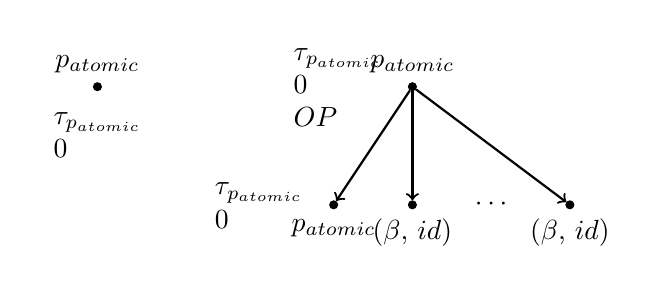
\begin{tikzpicture}[yscale=-1,
place/.style={circle,draw=black, fill=black, inner sep=0pt, 
              minimum size=1mm}]

	\node[place] (1st) at (1, 0) [label=above: $p_{atomic}$,
                                      label=below:
            \begin{tabular}{l}
              $\tau_{p_{atomic}}$\\
              $0$\\
            \end{tabular}] {};

\begin{scope}[xshift=4cm]
  \node[place] (1st) at (1, 0) [label=above: $p_{atomic}$,
                                label=left: 
             \begin{tabular}{l}
              $\tau_{p_{atomic}}$\\
              $0$\\
              $OP$\\ 
             \end{tabular}
] {};
	\node[place] (2nd) at (0, 1.5) [label=below: $p_{atomic}$,
                                        label=left: 
             \begin{tabular}{l}
              $\tau_{p_{atomic}}$ \\
              $0$ \\
             \end{tabular}
]{};
        \node[place] (3rd) at (1, 1.5) [label=below: {($\beta$, $id$)}] {};
	\node[place] (4rd) at (3, 1.5) [label=below: {($\beta$, $id$)}] {}; 

	\node (dots) at (2,1.5) {$\cdots$};
	
	\draw[->, thick] (1st) -- (2nd);
	\draw[->, thick] (1st) -- (3rd);
        \draw[->, thick] (1st) -- (4rd);
\end{scope}


\end{tikzpicture}
\end{center}   

\begin{itemize}
 \item \textit{Atomic predicate}

Suppose that $p_a$ is a \textit{atomic predicate}. Its type is $\tau$. The identity for some $OP$ associated with $p_a$ is $\beta$. 

The corresponding tree of it is a node $N_{p_a}$ with information, which are $\tau$ of $p_a$ and a number $0$, indicating that $p_a$ is atomic predicate. There are no branches for the node $N_{p_a}$. 

With the equivalence extension, the corresponding tree is presented in figure \ref{fig:APT}. The root is a node $N_{p_a}$ with information, which are the \textit{type} of $p_a$ $\tau$, the operation $OP$ and atomic mark $0$. The branches are a node $N'_{p_a}$ and several nodes $N_{\beta}$.  $N'_{p_a}$ carries information $\tau$, which is $p_a$'s type and atomic mark $0$. $N_{\beta}$ carries information of identity $\beta$ and identity mark $id$, the number of such nodes depends on two comparing predicates.

% pictures
\begin{figure}[h!]
\begin{center}
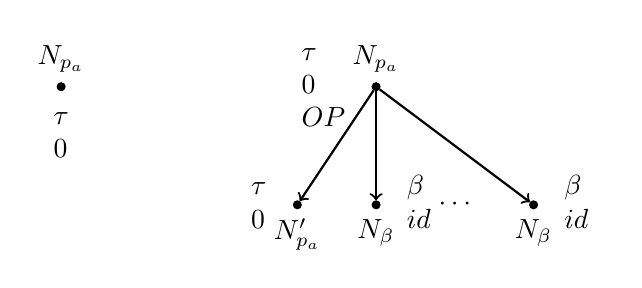
\begin{tikzpicture}[yscale=-1,
place/.style={circle,draw=black, fill=black, inner sep=0pt, 
              minimum size=1mm}]

	\node[place] (1st) at (1, 0) [label=above: $N_{p_a}$,
                                      label=below:
            \begin{tabular}{l}
              $\tau$\\
              $0$\\
            \end{tabular}] {};

\begin{scope}[xshift=4cm]
  \node[place] (1st) at (1, 0) [label=above: $N_{p_a}$,
                                label=left: 
             \begin{tabular}{l}
               $\tau$\\
               $0$\\
               $OP$\\
             \end{tabular}
] {};
	\node[place] (2nd) at (0, 1.5) [label=below: $N'_{p_a}$,
                                        label=left: 
             \begin{tabular}{l}
              $\tau$ \\
              $0$ \\
             \end{tabular}
]{};
        \node[place] (3rd) at (1, 1.5) [label=below: $N_{\beta}$,
        							  label=right: 
             \begin{tabular}{l}
              $\beta$ \\
              $id$ \\
             \end{tabular}        
        ] {};
	\node[place] (4rd) at (3, 1.5) [label=below: $N_{\beta}$,
							  label=right: 
             \begin{tabular}{l}
              $\beta$ \\
              $id$ \\
             \end{tabular}
	] {}; 

	\node (dots) at (2,1.5) {$\cdots$};
	
	\draw[->, thick] (1st) -- (2nd);
	\draw[->, thick] (1st) -- (3rd);
         \draw[->, thick] (1st) -- (4rd);
\end{scope}


\end{tikzpicture}
\end{center}   
\caption{Atomic predicate tree with equivalence}
\label{fig:APT}
\end{figure}

 \item \textit{Complex predicate}

For \textit{complex predicate}, there would be at least one rule defining it as,
\[p_c(\vec{t}) \stackrel{c,F_c}{\longleftarrow}F(p_1(\vec{t_1}),...,p_n(\vec{t_n}))\]
and for $OP=(\hat{F_c},\hat{F})$, there exists an identity $\alpha$.  $\tau$, and $\tau_{i}$ are represented types of $p_c$ and $p_{i}$ respectively.

The corresponding tree for $p_c$ is

% pciture
\begin{center}
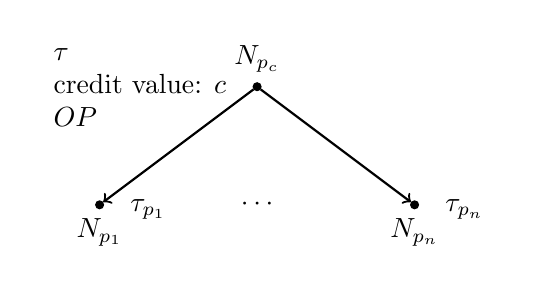
\begin{tikzpicture}[yscale=-1,
place/.style={circle,draw=black, fill=black, inner sep=0pt, 
              minimum size=1mm}]

  \node[place] (1st) at (2, 0) [label=above: $N_{p_c}$,
                                label=left: 
             \begin{tabular}{l}
               $\tau$\\
               credit value: $c$\\
               $OP$\\
             \end{tabular}
] {};
	\node[place] (2nd) at (0, 1.5) [label=below: $N_{p_1}$,
							  label=right: 
             \begin{tabular}{l}
            $\tau_{p_1}$\\
             \end{tabular}
	] {};
        \node[place] (3rd) at (4, 1.5) [label=below: $N_{p_n}$,
        							label=right: 
             \begin{tabular}{l}
             $\tau_{p_n}$ \\
             \end{tabular}        
        ] {}; 
	
	\node (dots) at (2,1.5) {$\cdots$};
	
	\draw[->, thick] (1st) -- (2nd);
	\draw[->, thick] (1st) -- (3rd);
        

\end{tikzpicture}
\end{center}   

where $N_{p_c}$ is the root with information which are $\tau$, $OP$ and credit value $c$. $N_{p_i}$s are the branches carrying their \textit{types} as information.

With the equivalence extension, the tree is 

% pictures
\begin{center}
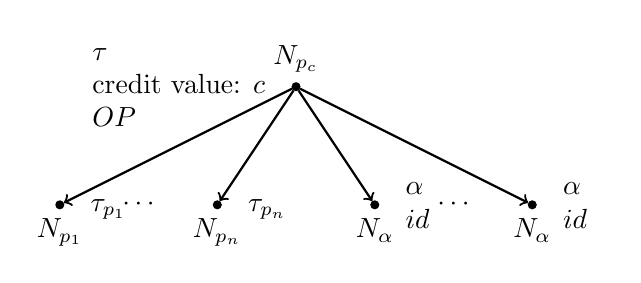
\begin{tikzpicture}[yscale=-1,
place/.style={circle,draw=black, fill=black, inner sep=0pt, 
              minimum size=1mm}]

  \node[place] (1st) at (3, 0) [label=above: $N_{p_c}$,
                                label=left: 
             \begin{tabular}{l}
               $\tau$\\
               credit value: $c$\\
               $OP$\\
             \end{tabular}
] {};
	\node[place] (2nd) at (0, 1.5) [label=below: $N_{p_1}$,
							label=right: 
             \begin{tabular}{l}
            $\tau_{p_1}$\\
             \end{tabular}
	] {};
	\node[place] (3rd) at (2, 1.5) [label=below: $N_{p_n}$,
							  label=right: 
             \begin{tabular}{l}
            $\tau_{p_n}$\\
             \end{tabular}
	] {}; 
        \node[place] (4rd) at (4, 1.5) [label=below: $N_{\alpha}$,
        						  label=right: 
             \begin{tabular}{l}
            $\alpha$\\
            $id$\\
             \end{tabular}
        ] {}; 
        \node[place] (5rd) at (6, 1.5) [label=below: $N_{\alpha}$,
        						  label=right: 
             \begin{tabular}{l}
            $\alpha$\\
            $id$
             \end{tabular}
	] {}; 

	\node (dots) at (1,1.5) {$\cdots$};
        \node (dots) at (5,1.5) {$\cdots$};
	
	\draw[->, thick] (1st) -- (2nd);
	\draw[->, thick] (1st) -- (3rd);
        \draw[->, thick] (1st) -- (4rd);
        \draw[->, thick] (1st) -- (5rd);
\end{tikzpicture}
\end{center}   
 $N_{p_c}$ is the root with information which are $\tau$, $OP$ and credit value $c$. $N_{p_i}$s are the branches with their \textit{types} as information, and several nodes $N_{\alpha}$ carrying information of identities $\alpha$ with identity mark $id$ are added as extra branches depending on two comparing predicates.
\end{itemize}

\begin{ex}
Continuation of the example \ref{ConstructPredicateTree}, reconstruct predicate trees with equivalence.

\begin{center}
\begin{tabular}{l l}
$has\_tasty\_food:$  & $(Restaurant)$\\

$has\_healthy\_food:$ &  $(Restaurant)$\\

$has\_good\_service:$  & $(Restaurant)$\\

$tasty\_restaurant:$  & $(Restaurant)$\\

$good\_restaurant:$  & $(Restaurant)$\\
\end{tabular}
\end{center}
\begin{tabular}{l l l}
$tasty\_restaurant(X)$ & $\stackrel{1.0,.}{\longleftarrow} prod$ & $has\_tasty\_food(X)$\\

$good\_restaurant(X)$ & $\stackrel{0.8,.}{\longleftarrow} prod$ & $has\_healthy\_food(X), has\_good\_service(X)$ \\
\end{tabular}

The predicate tree for \textit{has\_tasty\_food} is represented in figure \ref{fig:ex1}.
\begin{figure}[h!]
\begin{center}
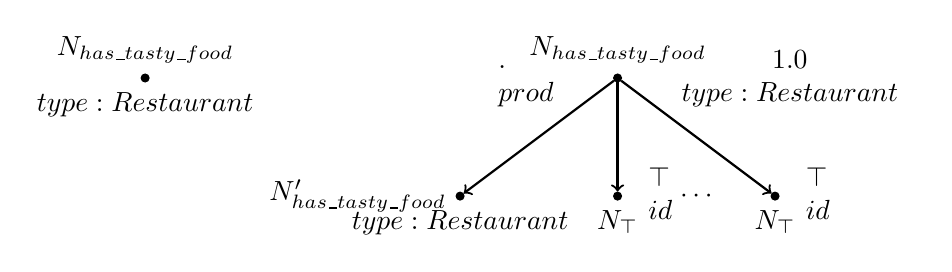
\begin{tikzpicture}[yscale=-1,
place/.style={circle,draw=black, fill=black, inner sep=0pt, 
              minimum size=1mm}]

 \node[place] (1st) at (0, 0) [label=above: $N_{has\_tasty\_food}$,
                               label=below: $type : Restaurant$] {};
	

\begin{scope}[xshift=4cm]
  \node[place] (1st) at (2, 0) [label=above: $N_{has\_tasty\_food}$,
                                label=right: 
       \begin{tabular}{l c}
         & $1.0$\\
         & $type : Restaurant$ \\
       \end{tabular},
       label=left:
       \begin{tabular}{l l}
         $.$ &\\
         $prod$ &\\
       \end{tabular}] {};
  \node[place] (2nd) at (0, 1.5) [label=left: $N'_{has\_tasty\_food}$,
                                  label=below: $type : Restaurant$] {};
  \node[place] (3rd) at (2, 1.5) [label=below: $N_{\top}$,
  						  label=right: 
             \begin{tabular}{l}
            $\top$\\
            $id$\\
             \end{tabular}
	]{}; 

  \node[place] (4th) at (4, 1.5) [label=below: $N_{\top}$,
    						  label=right: 
             \begin{tabular}{l}
            $\top$\\
            $id$\\
             \end{tabular}
  ]{};

  \node (dots) at (3,1.5) {$\cdots$};

  \draw[->, thick] (1st) -- (2nd);
  \draw[->, thick] (1st) -- (3rd);
  \draw[->, thick] (1st) -- (4th);
\end{scope}

\end{tikzpicture}
\end{center}   
\caption{two equivalent predicate trees for has\_tasty\_food}
\label{fig:ex1}
\end{figure}

The predicate tree for \textit{tasty\_restaurant} is represented in figure \ref{fig:ex2.1}, and \ref{fig:ex2.2} which is extended with equivalence.
\begin{figure}[h!]
\begin{center}
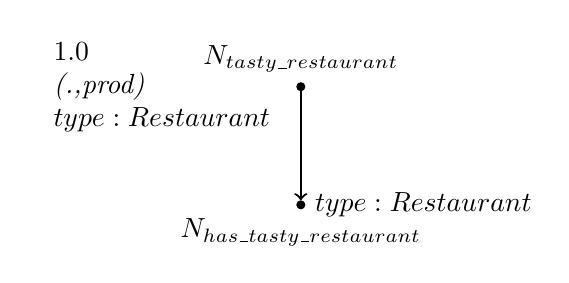
\begin{tikzpicture}[yscale=-1,
place/.style={circle,draw=black, fill=black, inner sep=0pt, 
              minimum size=1mm}]

\node[place] (1st) at (0, 0) [label=above: $N_{tasty\_restaurant}$,
                              label=left: 
             \begin{tabular}{l}
               $1.0$\\
               \textit{(.,prod)}\\
               $type : Restaurant$\\
             \end{tabular}
] {};
\node[place] (2nd) at (0, 1.5) [label=below:  $N_{has\_tasty\_restaurant}$,
label=right: 
$type : Restaurant$] {};
        
	\draw[->, thick] (1st) -- (2nd);
	
\end{tikzpicture}
\end{center}
\caption{predicate tree for tasty\_restaurant}
\label{fig:ex2.1}   
\end{figure}
\newpage
\begin{figure}
\begin{center}
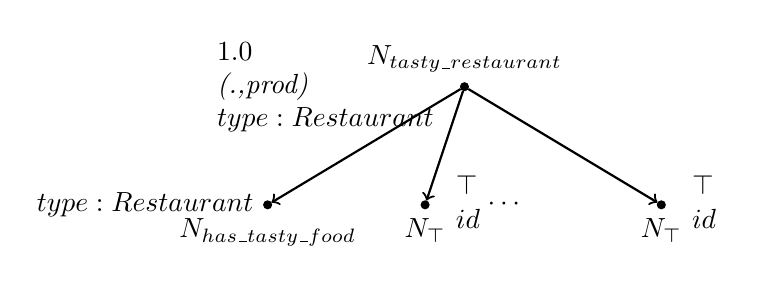
\begin{tikzpicture}[yscale=-1,
place/.style={circle,draw=black, fill=black, inner sep=0pt, 
              minimum size=1mm}]

  \node[place] (1st) at (2.5, 0) [label=above: $N_{tasty\_restaurant}$,
                                label=left: 
             \begin{tabular}{l}
               $1.0$\\
               \textit{(.,prod)}\\
               $type : Restaurant$\\
             \end{tabular}
] {};
	\node[place] (2nd) at (0, 1.5) [label=below: $N_{has\_tasty\_food}$, 
        label=left: $type : Restaurant$] {};
        \node[place] (3rd) at (2, 1.5) [label=below: $N_{\top}$,
          						  label=right: 
             \begin{tabular}{l}
            $\top$\\
            $id$\\
             \end{tabular}
             ] {}; 
        \node[place] (4rd) at (5, 1.5) [label=below: $N_{\top}$,
          						  label=right: 
             \begin{tabular}{l}
            $\top$\\
            $id$\\
             \end{tabular}
             ] {}; 

        \node (dots) at (3,1.5) {$\cdots$};
	
	\draw[->, thick] (1st) -- (2nd);
        \draw[->, thick] (1st) -- (3rd);
        \draw[->, thick] (1st) -- (4rd);
\end{tikzpicture}
\end{center}   
\caption{predicate tree for tasty\_restaurant with equivalence extension}
\label{fig:ex2.2}
\end{figure}
\end{ex}

